\documentclass[reprint,aps,pra,superscriptaddress,
amsmath,amssymb]{revtex4-1}
\usepackage{mathtools}
\usepackage{graphicx}
\usepackage{booktabs,multirow}
\usepackage{braket}
\usepackage{textcomp}
\usepackage{yfonts}
\usepackage[
  bookmarks=false,
  %bookmarks=true,
  colorlinks,
  linkcolor=blue,
  urlcolor=blue,
  citecolor=blue,
  plainpages=false,
  pdfpagelabels,
  final,
  breaklinks=true
]{hyperref}

\begin{document}
\newcommand{\pd}[2]{\frac{\partial #1}{\partial #2}} 
% for partial derivatives
\newcommand{\td}[2]{\frac{d #1}{d #2}} 

\newcommand{\bs}{\boldsymbol}
\newcommand{\bt}{\textbf}
\newcommand{\sech}{\text{sech}}
\newcommand{\erfc}{\text{erfc}}
\newcommand{\bse}{\begin{subequations}}
\newcommand{\ese}{\end{subequations}}
\newcommand{\im}{\text{i}}
\newcommand{\ud}[0]{\mathrm{d}}
\newcommand{\norm}[1]{\left\lVert#1\right\rVert}
\newcommand{\op}{\widehat}

\graphicspath{{figures/},{../figures/}} % specifies the path for the figures
\allowdisplaybreaks

\title{Retrieval of birefringent and scalar pupils from stacks of 
blurred point-spread functions generated by fluorescent nanobeads}
%   Characterizing birefringent pupils in widefield fluorescence 
% microscopy using phase retrieval}
\author{R. Guti\'{e}rrez-Cuevas}
\email{rodrigo.gutierrez-cuevas@fresnel.fr}
\affiliation{Aix Marseille Univ, CNRS, Centrale Marseille, Institut Fresnel, UMR 7249, 13397 Marseille Cedex 20, France}
\affiliation{Institut Langevin, ESPCI Paris, Université PSL, CNRS, 
75005 Paris, France}

\date{\today}

\begin{abstract}
Here we present the theory and the different strategies for retrieving the 
pupil of in fluorescence microscopy where the effects of birefringence play 
an  important role. We also study the effect of separating the signal into 
different polarization channels.
\end{abstract}


\pacs{}

\maketitle

%----------------------------------------------------------------------------
%---------------------------Introduction-------------------------------------
%----------------------------------------------------------------------------

\section{Intro}

General intro about fluorescence microscopy, SMOLM and PSF engineering.
Finish by saying something along the lines of:
However, any aberration or misalignment in the system can affect the 
final shape of the PSFs and thus lead to an inaccurate estimate of the 
parameters. 

A common solution to this problem is to perform a set of calibration 
measurements with a known source and at varying focal planes 
\cite{hanser2003phase,hanser2004phase}. From 
these measurements and an accurate model for the propagation of the light
emitted by the source to the camera, the aberrations can be estimated 
through phase retrieval algorithms. Initially, only scalar models with point 
sources were used which allowed the successful use of both iterative and 
nonlinear optimization routines for estimating the aberrations 
\cite{hanser2003phase,hanser2004phase,clark2012microscope}. However, 
more accurate models \cite{thao2019phase,ferdman2020vipr} take into 
account the vectorial nature of light which is essential to describe 
the propagation of the emitted radiation through the 
interface between the suspension medium and the immersion liquid used for 
the high-NA microscope objective \cite{novotny2006principles}. Moreover,
it is also necessary to consider that the most common sources, 
such as fluorescent nanobeads, emit 
incoherent light and their size can thus lead to a noticeable blurring of 
the PSFs.
Given these more accurate assumptions, 
iterative algorithms cannot be directly applied and have to be adapted which 
can make them unstable, although some success has been demonstrated 
\cite{thao2019phase}. A more natural approach is to use nonlinear optimization
\cite{fienup1982phase,ferdman2020vipr}
since it provides us with the freedom to incorporate other unknown parameters
into the estimation, such as the photobleaching amplitudes or the background 
illumination.

Up until now, all works have assumed a scalar pupil to characterize 
the aberrations or to design new PSFs. However, SMOLM requires the use 
of birefringent elements to encode the orientation information of the 
emitting dipole
into the shape of the two polarization components of the PSF. 
Therefore, it is important to update the model of propagation for an accurate
characterization or design of SMOLM systems. In this work, we propose a 
characterization technique and algorithm to estimate the polarization aberrations 
of the system \cite{hansen1988overcoming} as well as other unknown (or poorly known) parameters. 
This is done by applying a nonlinear optimization algorithm to a physical model
where the aberrations (or widow we want to design) are now represented by a Jones
matrix. The implementation is done with the 
neural network framework \texttt{PyTorch} \cite{} which performs automatically
all the gradient computation \cite{}. Additionally, we show that, in general,
it is necessary to introduce polarization diversity in the measurements 
in order to properly characterize the polarization response. This is similar 
to the introduction of phase diversity by taking images at various focal planes.
Additionally, we implement the most useful method for taking into account the 
blurring to the size of the nanobead discussed in \cite{}.
It should also be noted that all the results obtained in this work 
were achieved with the software \texttt{torchPSFstack} which is freely 
accessible at \cite{}.

% This is the goal of this work 
% where we define a phase retrieval algorithm to retrieve the Jones matrix at 
% the BFP that accounts for all the imperfections in the system. The approach 
% is base on the assumptions of an incoherent point source, which is the case 
% for fluorescent nanobeads used for most characterizations, and the use of 
% both phase and polarization diversities. The phase diversity is the standard 
% approach of taking several images across several focal planes and the 
% polarization diversity is obtained by using a polarization analyzer. Moreover, 
% given several measurements across the field it will also be possible to 
% determine the field dependent polarization aberrations 
% \cite{zheng2013characterization}.


% In general terms the goal of phase retrieval is to estimate the phase of a 
% field given a set of intensity measurements. In imaging applications, the 
% spatial distribution of a given object can then be reconstructed from the 
% complete information of the field. The different intensity measurements can 
% be performed at different focal or image planes, or even under varying 
% illumination conditions. In the particular case of fluorescence microscopy 
% \cite{moerner2003methods}, the objective is to retrieve the field 
% distribution at the back-focal plane (BFP) from intensity measurements of 
% the point-spread function at varying focal planes 
% \cite{hanser2003phase,hanser2004phase}. In this case it might be more 
% adequate to call the task pupil retrieval since we are looking for both 
% the phase and amplitude at the BFP. But, following common practice we will 
% use them interchangeably since the field at the BFP is linked to the one 
% at the image plane via a scaled Fourier transformation so, in principle, 
% complete knowledge from one entails complete knowledge of the other.

% The most common and best known method for phase retrieval is the iterative 
% Gerchberg-Saxton (GS) algorithm which is an iterative approach performed by 
% Fourier transforming back and forth from the BFP to the image plane 
% \cite{shechtman2015phase}. Depending on the particular setup and application, 
% it might also be possible to use intensity measurements at the BFP and at 
% various focal or image planes which can help the convergence of the 
% algorithm. One great advantages of the GS algorithm is that it is fast 
% and easy to implement. Moreover, it provides an estimate for the intensity 
% distribution at the Fourier plane (if it is not given). However, it is not 
% directly applicable to every situation and might not provide the best 
% estimate. This is the reason why phase retrieval algorithms have moved 
% away from the iterative approach of the GS algorithm and into the domain 
% of nonlinear optimization routines \cite{fienup1982phase}. 
% This latter approach provides a lot of freedom since any experimental 
% parameter that is not perfectly known can be estimated. 

% In fluorescence microscopy, phase retrieval algorithms are used to estimate 
% the aberrations and imperfections of the experimental setup. A good estimate 
% is essential since it can have drastic effects on the shape of the intensity 
% distribution of the PSF which is used to encode additional information about 
% the emitter, such as its longitudinal position 
% \cite{moerner2003methods,curcio2020birefringent}. Both iterative and 
% nonlinear optimization routines have been used successfully 
% \cite{hanser2003phase,hanser2004phase,clark2012microscope}. The standard 
% approach has been to assume a fully scalar model and it is only recently that 
% the true vector nature of the dipolar emitters has been taken into account  
% \cite{thao2019phase,ferdman2020vipr}. The vector nature is essential to 
% accurately model the propagation of the emitted radiation through the 
% interface between the suspension medium and the immersion liquid used for 
% the high-NA microscope objective. 

% Lately, the PSF shaping technique has been extended to encode the 
% orientation of the emitting dipoles by translating the polarization 
% distribution of the dipolar radiation into the shape of the PSF  
% \cite{curcio2020birefringent} . This is inevitably done by polarization 
% optics and birefringent element which have and are more sensitive to 
% polarization aberrations. It is therefore essential to take them into 
% account for an accurate modeling of the PSFs. This is the goal of this work 
% where we define a phase retrieval algorithm to retrieve the Jones matrix at 
% the BFP that accounts for all the imperfections in the system. The approach 
% is base on the assumptions of an incoherent point source, which is the case 
% for fluorescent nanobeads used for most characterizations, and the use of 
% both phase and polarization diversities. The phase diversity is the standard 
% approach of taking several images across several focal planes and the 
% polarization diversity is obtained by using a polarization analyzer. Moreover, 
% given several measurements across the field it will also be possible to 
% determine the field dependent polarization aberrations 
% \cite{zheng2013characterization}.



\section{Modeling the PSFs for fluorescence microscopy}

\subsection{Field at the back-focal plane}

\begin{figure*}
  \centering
  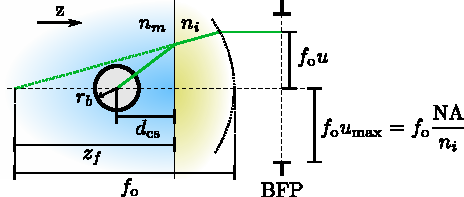
\includegraphics[width=.9\linewidth]{aplanatic.pdf}
  \caption{\label{fig:setup} Schematic of the experimental setup for the 
  collection and shaping of the emission by a source. (left) Schematic of the position 
  source, in this case represented by a fluorescent nanobead, with respect
  to the interface between the embedding medium of index of refraction
  $n_i$ with the immersion medium of index of refraction $n_f$ used for 
  the high-NA microscope objective and of the focal plane. (right) 
  Schematic of the collection arm composed of a microscope objective (MO), 
  followed by a birefringent mask (BM) and a polarization analyzer (PA). 
  The light at the BFP is then focused onto the camera by the tube lens 
  of focal length $f_\text{tl}$. }
\end{figure*}

The first step is to have the most accurate model for the propagation 
of light through our microscope. As shown in Fig.~\ref{fig:setup}, 
the source is embedded in a medium of index of refraction $n_i$ at a 
distance $z_0$ from the interface with immersion oil of index of 
refraction $n_f$, the interface is given by the coverslip which is assumed
to be index matched to the immersion oil. For a dipolar source, the green 
tensor at the back-focal plane (BFP) of a high-NA objective can be 
computed through Richards-Wolf diffraction 
theory for aplanatic systems \cite{richards1959electromagnetic,
novotny2006principles}. An important step in this calculation is to  
take into account the interface between the two media since it introduces 
spherical aberration and the coupling of evanescent waves when $n_f > n_i$,
known as supercritical angle fluorescence (SAF), 
which  can contribute to more than 
half of the radiation reaching the detector \cite{hellen1987fluorescence,
axelrod2001total,axelrod2013evanescent}.

Following \cite{lieb2004single,novotny2006principles} and assuming that 
light propagates along the positive $\hat z$ direction, the Green tensor 
at the BFP,
\begin{align} \label{eq:G0}
\bt G (\bt u; \bt r_0) = &   e^{-\im k n_f \bs \rho_o \cdot \bt u } 
\exp \left[\im k n_i |z_0| 
\sqrt{1 - \left(\frac{n_f u}{n_i} \right)^2 } \right]  \nonumber \\
& \times \exp \left(\im k n_f z_f \sqrt{1 - u^2} \right) \bt g (\bt u) ,
\end{align}
where 
\begin{align}
\bt g (\bt u) =
\left(
\begin{array}{ccc}
g_{xx}  (\bt u)& g_{xy}  (\bt u)& g_{xz}  (\bt u) \\
g_{yx}  (\bt u)& g_{yy}  (\bt u)& g_{yz} (\bt u)
\end{array}
\right)
\end{align}
with the explicit form of  its components given in the Appendix, 
$\bt r_0=\bs \rho_0 + \hat{\bt z} z_0$ is the position of the source
with $\bs \rho_0 =(x_0,y_0)$  denoting its transverse location, 
$k=2 \pi/\lambda$ with $\lambda$ being the wavelength,
and 
$z_f$ is the location of the focal plane from the interface, $z_f<0$ 
($z_f>0$) if the focal plane is in the medium with index of refraction 
$n_i$ ($n_f$). The vector 
$\bt u = (u_x, u_y)$ denotes the normalized coordinates at the BFP, 
see Fig.~\ref{fig:setup}. The maximum value of $u = \norm{\bt u}$ is 
limited by the NA through $u_\text{max} = \text{NA}/n_f$. 
The matrix elements $g_{ij}$ include the effect of the Fresnel coefficients 
of the boundary and depend on $\bt u$ but not on the location of the dipole 
or the focal plane.  For a dipole oriented along the unit vector 
$\bs \mu = (\mu_x, \mu_y, \mu_z)$, the electric field distribution at the BFP 
is given by 
\begin{align}
\bt E (\bt u; \bt r_0) = \bt G (\bt u; \bt r_0) \cdot \bs \mu.
\end{align}
Therefore, the three columns of the Green tensor represent the field 
distribution produced by a dipole along each of the three coordinate axes. 


\subsection{Propagation from the BFP to the image plane}


In order to encode information about the position and orientation of the 
dipole into the shape of the PSF, it is necessary to include a mask into the 
path of the emitted light at the BFP with the possible help a relay system 
as shown in Fig.~\ref{fig:setup}. 
The most general case is that of a 
birefringent mask represented by a $2\times 2$ Jones matrix \cite{},
\begin{align} \label{eq:jqw}
\bt J_\text{M}(\bt u) =  \left(
\begin{array}{cc}
J_{xx}&J_{xy} \\
J_{yx} & J_{yy}
\end{array}
\right).
\end{align}
Note that a scalar mask case with apodization is regained if $q_j=0$ 
for $j=1,2,3$, and a pure phase mask if also $q_0 =1$.
After multiplying the Green tensor by this Jones matrix, the field  can then 
be propagated form the BFP to the image plane through
\begin{align}
\bt G_\text{IP} (\tilde{\bs \rho}; \bt r_0 ) = \iint  \bt J_\text{M}(\bt u)  
\cdot \bt G_0  (\pm \bt u,; \bt r_0) e^{- \im k  \frac{n_f \tilde{\bs \rho}}{M}  \cdot \bt u } \ud \bt u ,
\end{align}
where $\tilde{\bs \rho}$ denotes the transverse position at the image plane, and
$M$ is the total magnification of the system. 
Note that the normalized coordinate is defined at the location of the birefringent  mask.
Assuming an incoherent source, the PSF is then given by
\begin{align}
  I_\text{IP} (\tilde{\bs \rho}; \bt r_0) =  \norm{\bt G_\text{IP} }^2 
  = \sum_{i=x,y} \sum_{j=x,y,z} |G_{\text{IP},ij}( \bt u)|^2.
\end{align}

\section{Modeling for the phase retrieval}

\subsection{Polarization aberrations}

The decomposition of polarization aberrations by a Jones matrix can be 
done in the following manner
\begin{align} \label{eq:jqw}
  \bt J_\text{A}(\bt u) = e^{\im 2\pi W(\bt u)} \left(
\begin{array}{cc}
q_0(\bt u) + \im q_3(\bt u) &q_2(\bt u) + \im q_1(\bt u) \\
-q_2(\bt u) + \im q_1(\bt u) & q_0(\bt u) - \im q_3(\bt u)
\end{array}
\right),
\end{align}
which allows separating the scalar aberrations, contained 
in $W$ from the vectorial correction given by the $q$'s. 
Since aberrations tend to be described by smooth functions, it generally 
suffices to decompose the various elements of the Jones matrix using the 
Zernike polynomials which constitute a complete basis on the unit disk.
Therefore, we write
\begin{align}
  W (\bt u) = &\sum'_l c_{l}^{(W)} Z_l(\bt u/u_\text{max}) ,\\
  q_{j} (\bt u) = &\sum_l c_{l}^{(j)} Z_l(\bt u/u_\text{max}),
\end{align}
where $j=0,...,3$, and we used a single index notation for the basis. 
Note that $\sum'$ in the expression for $W$ indicates that the terms 
corresponding to piston and defocus should be excluded, this is 
automatically handled by the software \cite{}. The piston term only 
fixes a global phase which cannot be determined from intensity measurements
while the defocus term is redundant with the more accurate defocus parameter
$z_f$ in Eq.~\ref{eq:G0}. 
From now on, it will be assumed that the source is placed  
along the optical axis so that $\bs \rho_0 = (0,0)$, with
any deviation from this being corrected be the scalar tilts 
present in $W$.

This Zernike expansion is inspired by the Nijboer-Zernike theory 
\cite{janssen2002extended,braat2003extended,braat2005extended} where a 
scalar mask would be separated into real and imaginary parts before 
decomposing in terms of Zernike polynomials. 
Note that other models can be used, such as 
pixel by pixel decomposition, but a Zernike decomposition with enough 
terms should be able to handle most cases found in microscopes. Moreover, 
computationally there is no advantage to considering a pixel decomposition 
since the number of DFT (the most costly operation) would be the same.
It should also  be noted that a scalar mask can easily be modeled by just
setting the coefficients $c^{(j)}_l=0$ for all $l$ and $j=1,2,3$.


\subsection{Best focus and the distance to the coverslip}

In general the position chosen as the nominal focus (or best focus) $z_f$ and 
distance to the coverslip of the emitter $z_0$ are not perfectly 
known. Therefore,
it is worth considering them as part of the optimization parameters that 
will be estimated along with the coefficients of the Zernike decomposition 
of the birefringent mask. The most obvious solution is to directly 
use $z_f$ and $z_0$ as parameters, however both phase 
terms have similar effect when the 
radial coordinate $u$ is below the SAF radiation which might cause the 
nonlinear optimization to fall into a local minimum.
Therefore, it is best to 
consider instead
\begin{align}
\bt G (\bt u)  = D_{\delta, \Delta z_f} (\bt u) \bt g(\bt u),
\end{align}
where
\begin{align}
D_{\delta, \alpha} (\bt u)= & \exp \Bigg\{ 
  \im 2 \pi n_f  \delta \Bigg[ \frac{n_i}{n_f} 
  \sqrt{1 - \left(\frac{n_f u}{n_i} \right)^2 }
- \alpha \sqrt{1 - u^2} \Bigg]\Bigg\} \\
& \times \exp \Bigg(
  \im 2 \pi n_f \Delta z_f \sqrt{1 - u^2} \Bigg) , 
\end{align}
with $\delta = |z_0| / \lambda$ and $z_f =\Delta z_f -\alpha |z_0|$. 
The key difference is that $\alpha$ is a constant that is chosen to minimize 
root-mean squared wavefront error (or a similar metric)
over the range $u \in [0, n_i/n_f]$. 
The parameter $\delta$ now predominantly controls the amount of exponential 
decay for the SAF radiation while $\Delta z_f$ controls the defocus of the system.
The plane $\Delta z_f =0$ is where the spherical aberration induced by the 
interface is best compensated with a simple defocus. Nonetheless, this plane 
might not coincide with the nominal focal plane chosen during the experimental 
acquisition given that the choice of the best focus from the image on the camera is 
quite subjective. In the supplemental document, we provide common choices
for the best focus with the appropriate PSF for various distances to the coverslip.
These can be used to determine a better initial value for $Delta z_f$ by 
comparing them to the data acquired experimentally. 

Even though this new choice of parameters helps the algorithm to differentiate 
between the two effects, if some apodization is included in the model then this 
can mimic or compensate for the exponential decay controlled by $\delta$. 
Therefore, on must be careful when including $\delta$ in the optimization 
routine. For fluorescent nanobead samples it is safe to 
assume that they are all fixed to the coverslip so that their distance to the 
coverslip can be taken as their radius and thus $\delta$ can be taken off 
the optimization routine. Nonetheless, in all the numerical experiments a 
slight error (chosen randomly between $0$ and $20$nm) was introduced 
for the value of $z_0$, this error  did not affect the final estimation
of the pupil.


\subsection{Phase and polarization diversity}

In phase retrieval algorithms for optical microscopes, it is common 
practice to assume that we have access to a stack of intensity images 
at varying focal distances separated by $\Delta z_{\zeta}$ from the 
location of the best focus. This varying focal 
distances are taken into account by multiplying the Green tensor by 
the phase factor
\begin{align}
D^\zeta (\bt u) =  \exp \left[ \im k n_f \Delta z_\zeta  \sqrt{1 - u^2} \right] 
\end{align}
This additional information, referred to as phase diversity, helps the 
algorithm converge to an appropriate solution without falling into 
local minima and helps discriminate between the right and left phase vortices. 
These measurements are sufficient when the aberrations are taken as 
scalar, however when birefringence effects need to be taken into account 
it is necessary to implement a method to also provides information 
about the polarization state of the PSFs for each focal distance. 
This supplementary information can be obtained by inserting a polarization 
analyzer right after the 
birefringence mask (see Fig.~\ref{fig:setup}). This polarization analyzer 
can be composed of a combination of waveplates and polarizers where at least
one element can rotate in order to change the polarization projection of 
the output. This polarization diversity is modeled by a set of constant 
Jones matrices $\bt P^{(p)}$ that is applied after all other birefringent masks.
Therefore, the stack of Green tensors at the BFP is given by
\begin{align}
\bt G^{(\zeta ,p)}_\text{BFP} (\bt u) =  D^{(\zeta )} (\bt u) \bt P^{(p)} 
\cdot \bt J_\text{A}(\bt u) \cdot \bt J_\text{M}(\bt u) \cdot \bt G_0  (\bt u).
\end{align}
In this model $\bt J_\text{M}$ represents any known
birefringent mask into the nominal Green tensor which can have approximately known
parameters that can be incorporated into the optimization routine.
It is worth noting that while experimentally the polarization diversity happens at 
the BFP, computationally it is better to perform it at the image plane in 
order to avoid the computation of unnecessary DFTs.


\subsection{Modeling the total measured intensity}

To model the intensity measured by the camera, the Green tensor is first 
propagated to the image plane via,
\begin{align}
\bt G^{(\zeta ,p)}_\text{IP} (\bs \rho ) 
= \iint \bt G^{(\zeta ,p)}_\text{BFP} (\bt u)  
e^{ - \im k  \frac{n_f \bs \rho}{M}  \cdot \bt u } \ud \bt u .
\end{align}
Here, it will be assumed that the source emits fully unpolarized light. This 
is the case for fluorescent nanobeads which are commonly used to characterize or test 
fluorescence microscopes since they have a stronger signal than that emitted 
by single fluorescent molecules. In this case the measured intensity is 
given by the incoherent sum of the PSFs produced by dipoles oriented along 
each of the three Cartesian axes which is the same as the squared Frobenius 
norm of the Green tensor at the image plane 
\begin{align}
I^{(\zeta ,p)}_\text{IP} (\bs \rho ) = \norm{\bt G^{(\zeta ,p)}_\text{IP} }^2 
= \sum_{i=x,y} \sum_{j=x,y,z} |G^{(\zeta ,p)}_\text{IP,ij}( \bt u)|^2.
\end{align}
Depending on the size of the source it might be necessary to perform 
one of the blurring operations described in \cite{}. If a three-dimensional 
blurring is needed the computation of supplementary quantities will need to 
added to the forward model, for example, for the exact hard-sphere model 
we would also need to compute the total intensity for other values of $d_cs$.
The downside is that this would slow the algorithm considerably. 
However, as long as their 
diameter is smaller than 30nm one can safely skip this step.
More details about the blurring models implemented can be found in the 
Supplementary Information.

As a last step for computing the measured intensity, we also consider 
the effect of photobleaching of the fluorescent nanobeads and the background 
illumination. The photobleaching causes the number of photons emitted by the 
nanobead to diminish with time. Its effect can be taken into account by 
implementing an overall amplitude factor $\mathcal{A}^{(p,\zeta)}$
which depends on both the phase and polarization diversities. The background 
illumination is then added incoherently to the photobleached PSF stack. 
The simplest model is to assume that the background illumination is constant 
across each intensity image and determined by the term 
$\mathcal{B}^{(p,\zeta)}$. Therefore, the final total measured intensities 
of the ZP stack are given by 
\begin{align}
I^{(\zeta ,p)}_\text{tot} (\bs \rho )  
  =  a^{(p,\zeta)} I^{(\zeta ,p)}_\text{IP} (\bs \rho ) + b^{(p,\zeta)}.
\end{align}
It is possible to assume a more complicated model for the background 
illumination, such as a quadratic expansion \cite{aristov2018zola}. 

\subsection{Cost function}

The last piece we need to consider is the choice of a cost function that 
compares how good our modeled PSFs $I^{(\zeta ,p)}_\text{tot}$
are compared to the measured ones $I^{(\zeta ,p)}_\text{exp}$.
Under the absence of noise, any choice of cost function that has a minimum 
when the two quantities are the same should provide the same result. However,
noise is ever present in experimental measurements and thus needs to be taken
account. If the noise in the camera follows a Poisson distribution then the 
log-likelihood cost function,
\begin{align}
  \mathcal{C}_\text{LL} = \sum_{\zeta,p} \iint w(\bs \rho )\left\{ 
    I^{(\zeta ,p)}_\text{exp} (\bs \rho )
  \log \left[ I^{(\zeta ,p)}_\text{tot} (\bs \rho ) \right]
  - I^{(\zeta ,p)}_\text{tot} (\bs \rho )\right\} \ud^2 \bs \rho.
\end{align}
Whereas if it follows a Gaussian distribution then the sum of the squared 
difference is the most appropriate,
\begin{align}
  \mathcal{C}_\text{SS} = \sum_{\zeta,p} \iint w(\bs \rho )\left[
    I^{(\zeta ,p)}_\text{exp} (\bs \rho )
  - I^{(\zeta ,p)}_\text{tot} (\bs \rho )\right]^2 \ud^2 \bs \rho.
\end{align}
A window function $w$ has been introduced to represent the use of a finite
region at the image plane and to exclude bad pixels if there are any.
It is also worth making a technical note. In order for the choice of cost function 
to make sense we need to use as $I^{(\zeta ,p)}_\text{exp}$ the values that 
actually follows the assumed distribution. In general this means that the images
should not be denoised and that the offset of the camera should be removed.
A detailed description for the forward model can be found in the Supplementary 
Information as well as other considerations that need to be taken into account 
before launching the optimization routine. 

\begin{figure}
  \centering
  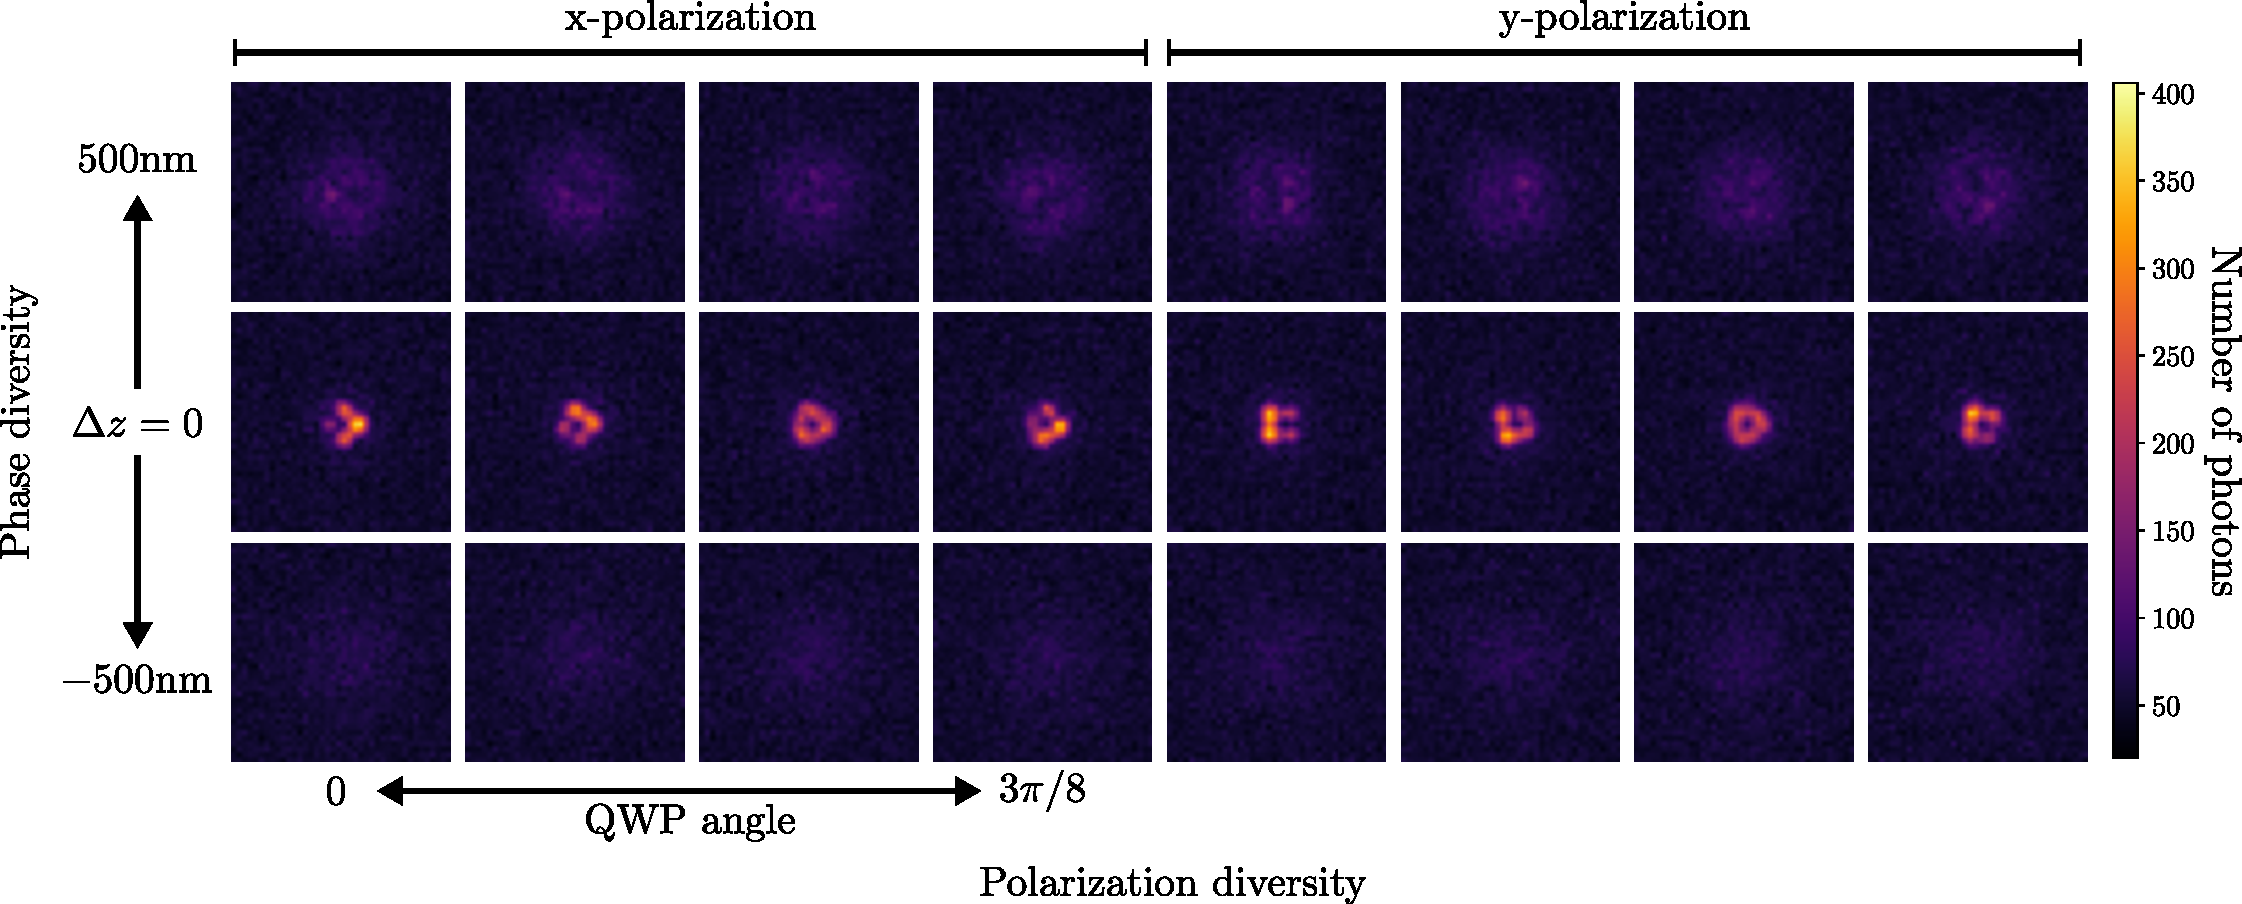
\includegraphics[width=1\linewidth]{stack_ex.pdf}
  \caption{\label{fig:stack} PSF stack with phase and polarization diversities 
  modelled with \texttt{pyPSFstack} and used for the retrieval of the Jones
  matrix of an SEO element. }
\end{figure}

\section{Numerical experiments}

To exemplify the implementation of the phase retrieval algorithm, 
two main birefringent masks will be considered: (2) a stress-engineered optical 
(SEO) element \cite{} and (3) an s-plate \cite{marrucci2006optical}. 
Both have been used in practice to measure
the position and orientation of dipolar emitters \cite{}. All the modelled
data stacks are computed using \texttt{pyPSFstack} which allows
computing the PSF stack with phase and polarization diversities, and can 
compute the three-dimensional blurring due to the size of the fluorescent
nano-bead. Figure \ref{fig:stack} shows as an example the stack used for 
retrieving the SEO birefringent mask with both phase and polarization diversity. 
It can also simulate the effect of the background illumination
and noise. The polarization diversity will be taken as the Jones matrix
given by a quarter-wave plate at various angles followed by a horizontal or 
vertical linear polarizer. This choice is inspired by the setup used in \cite{}
where the SEO is followed by a quarter-wave plate and then a Wollaston
prism separates the two linearly-polarized components. 

\subsection{Polarization diversity VS more phase diversity}

\begin{figure}
  \centering
  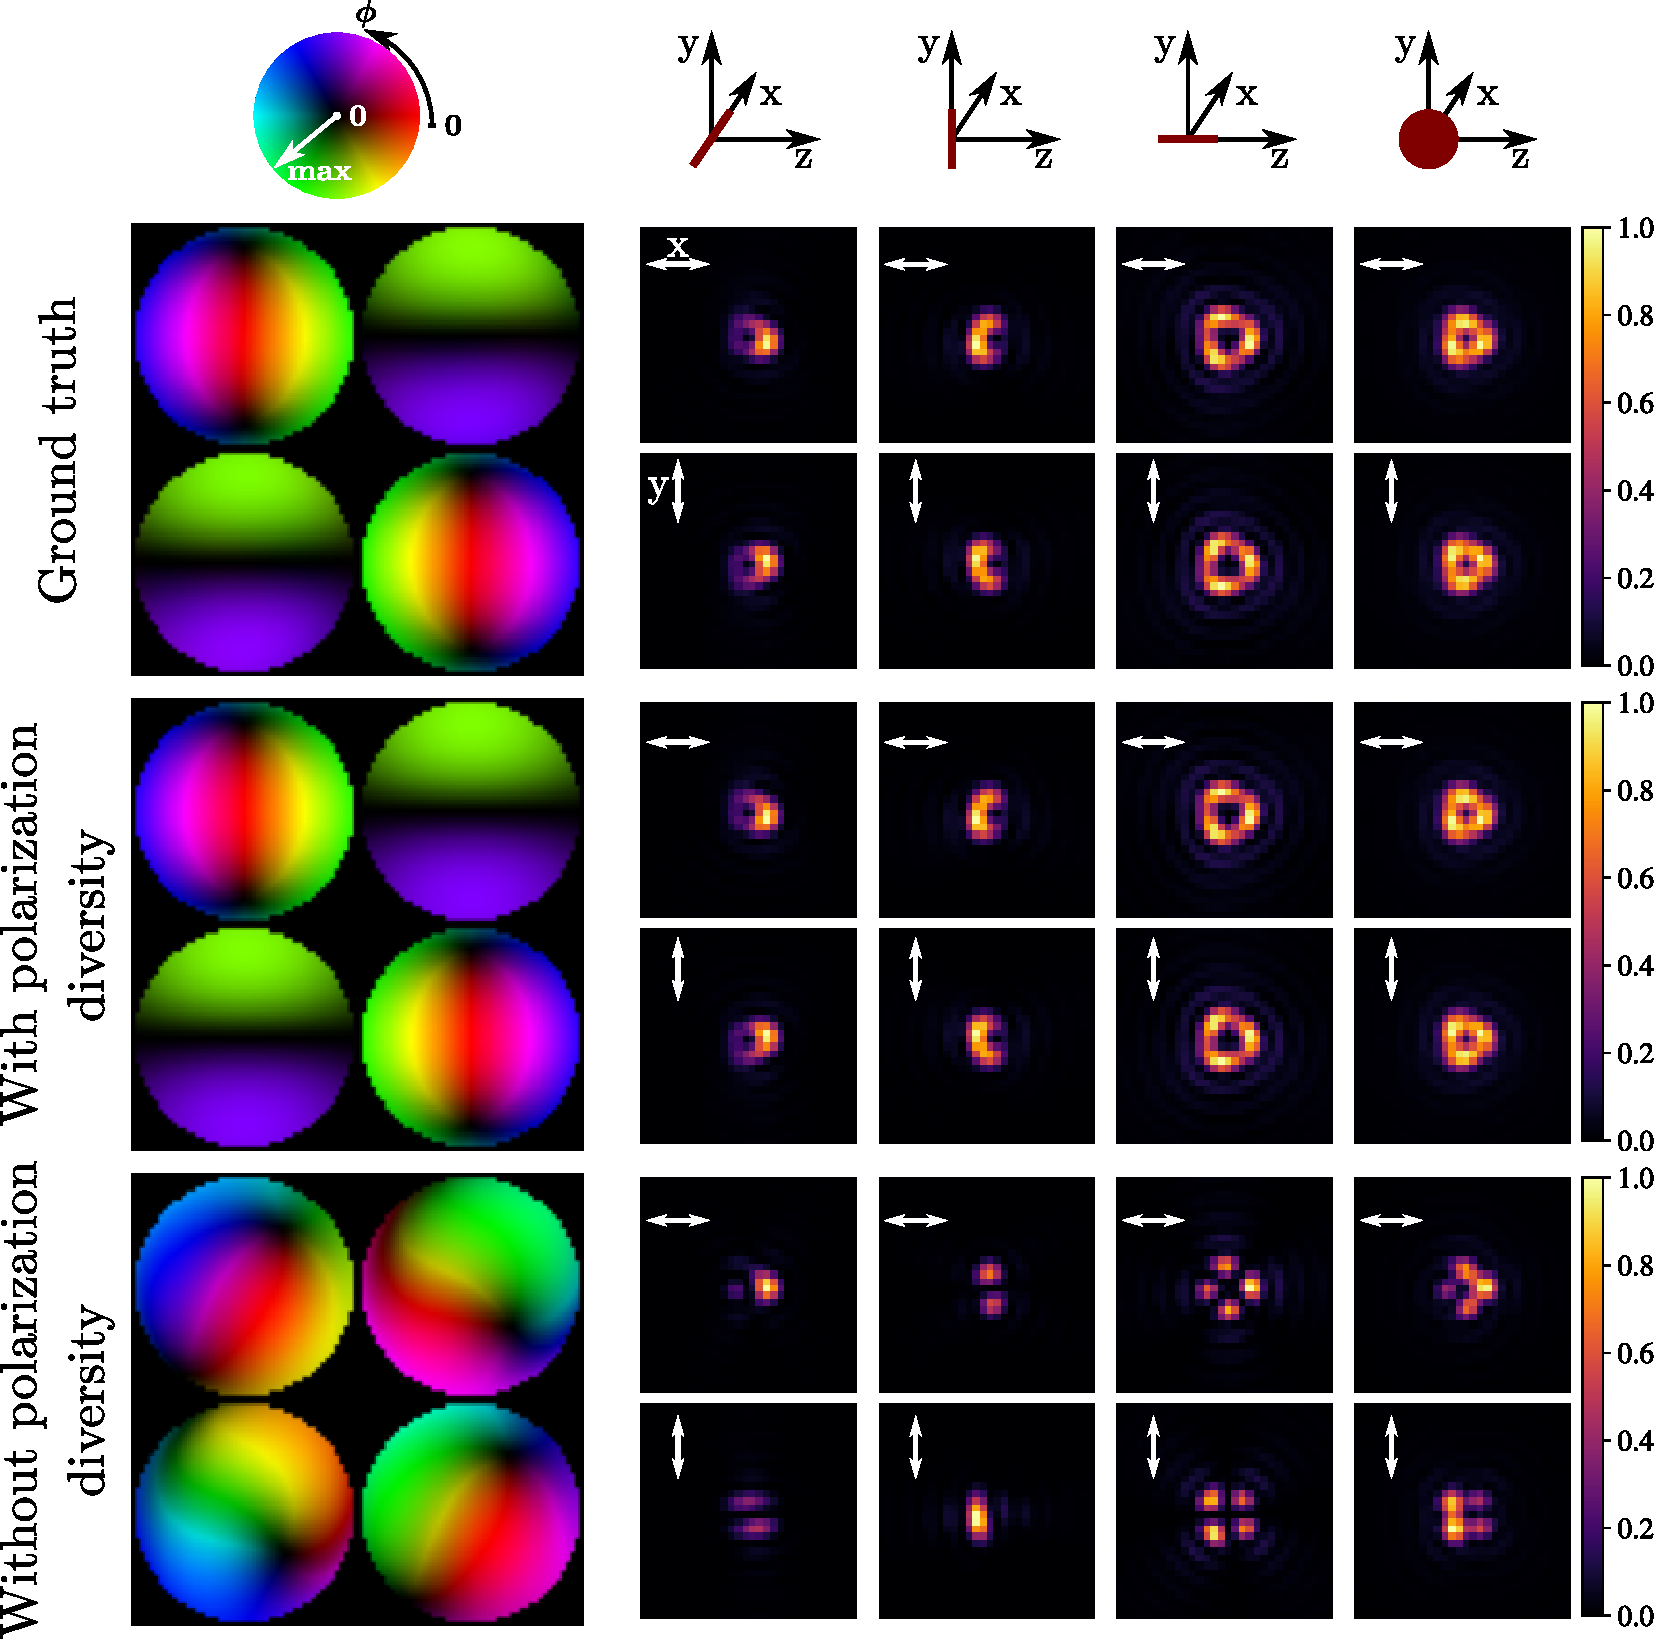
\includegraphics[width=1\linewidth]{seo_ret.pdf}
  \caption{\label{fig:seo_ret} . }
\end{figure}

\begin{figure}
  \centering
  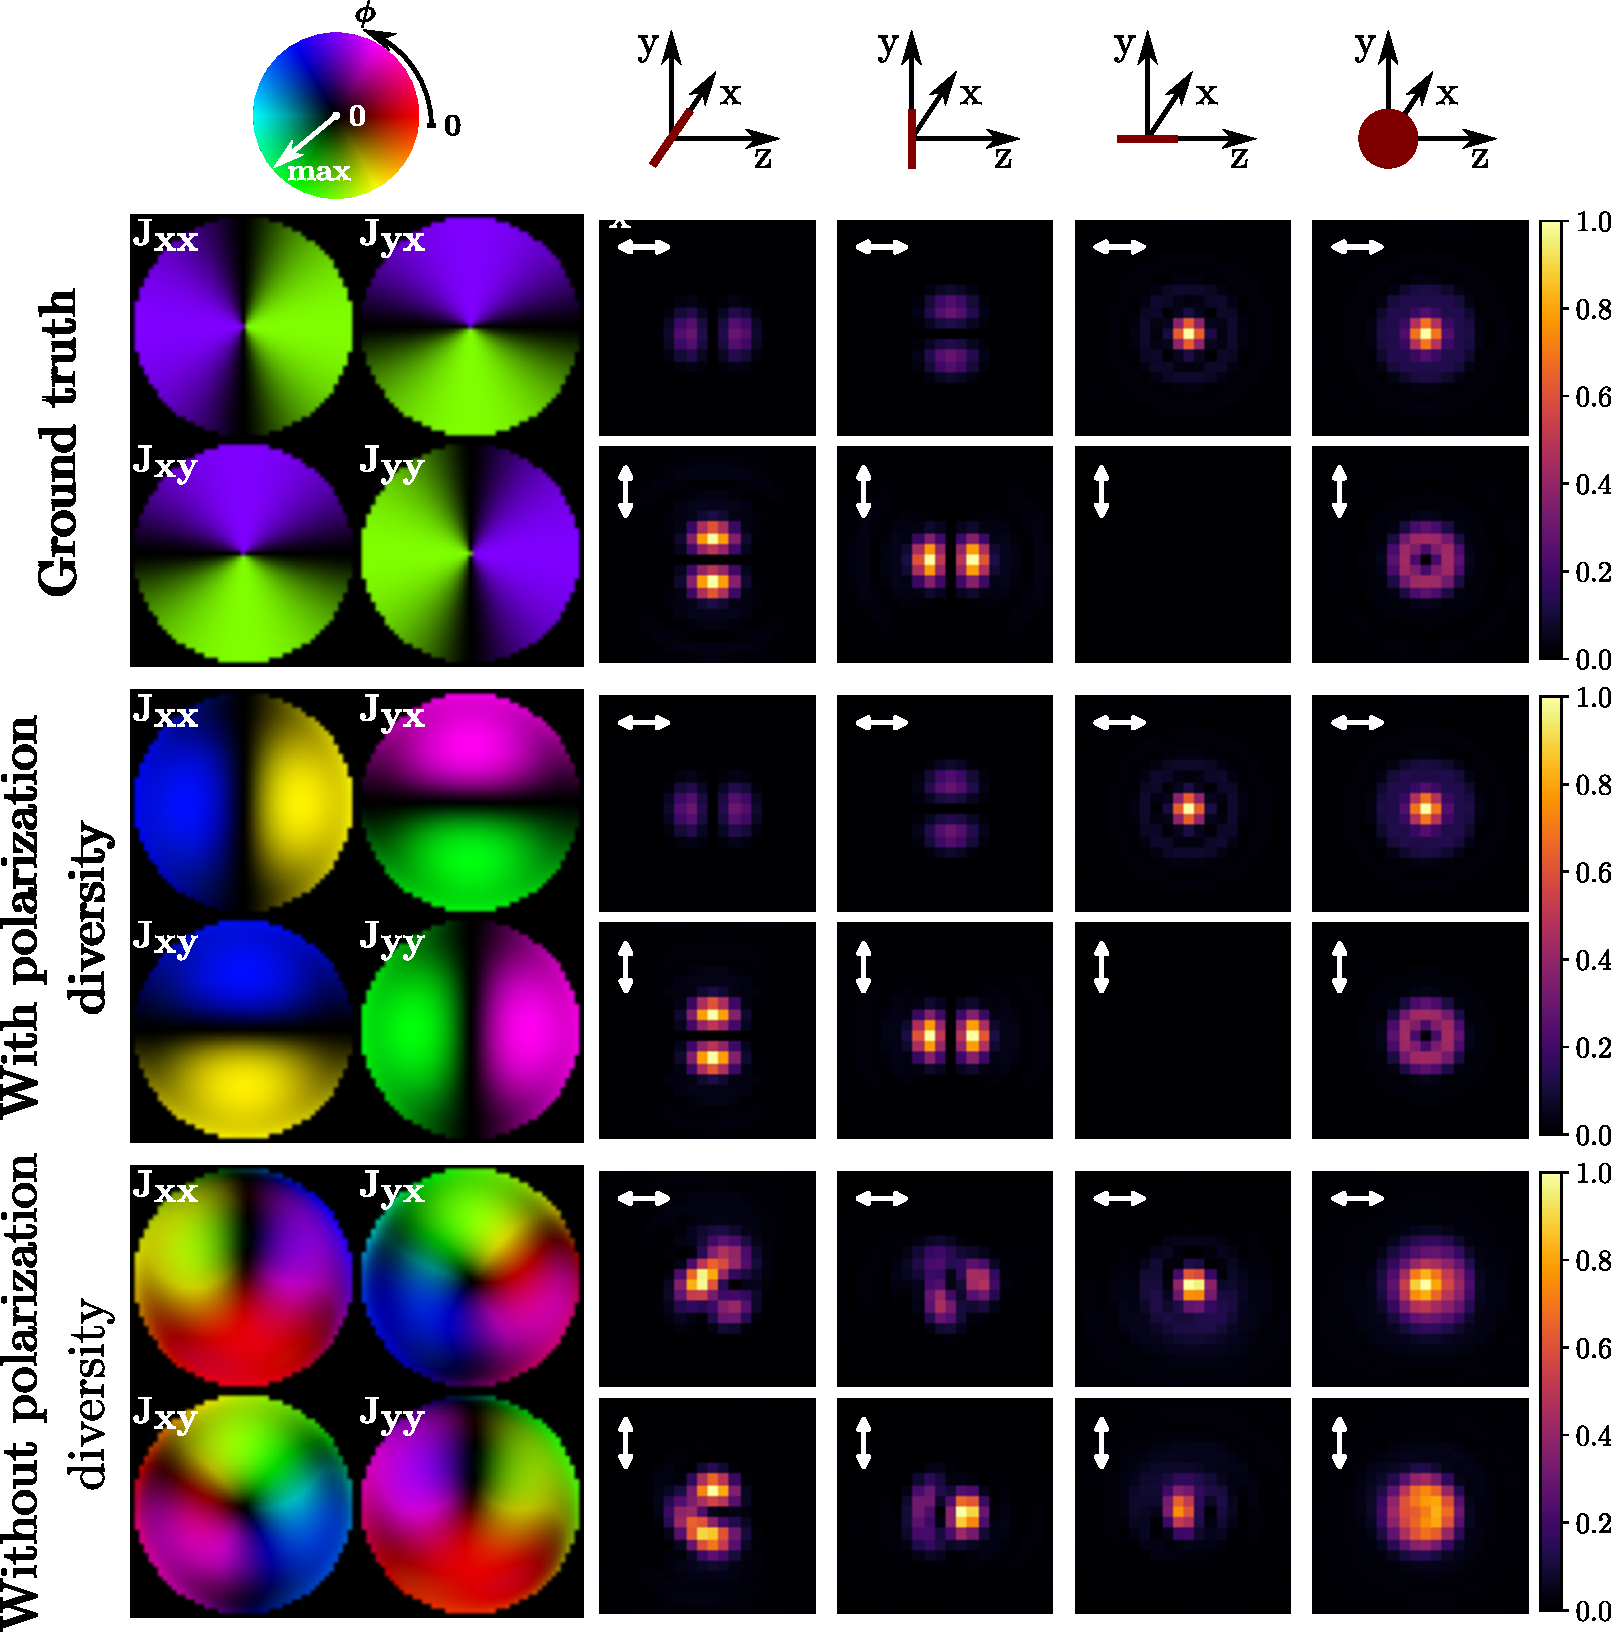
\includegraphics[width=1\linewidth]{qp_ret.pdf}
  \caption{\label{fig:qp_ret} . }
\end{figure}

As a first example, we consider the retrieval of a birefringent mask with and without
the use of polarization diversity. For this, the data is modelled assuming 
the source is a 20nm fluorescent nanobead,
with an average of 20000 photons hitting our detectors 
per PSF to which we add 100 photons per pixel 
as the background illumination. Noise following a Poisson distribution
is then added to the images. Note that the average number of photons on the 
PSFs measured with polarization diversity is halved due to the presence of a linear 
polarizer. Under these conditions, an image defocused by more 
than 500nm past the nominal focal plane will be indistinguishable from noise 
(see Fig.~\ref{fig:stack}). 
Therefore, for the phase diversity images are taken from -500nm to 500nm of the 
nominal focal plane with a step size of 100nm. For the polarization diversity, the 
quarter wave-plate is rotated from $0$ to $3\pi/8$ with a step of $\pi/8$ and is
then followed by a Wollaston prism which projects into horizontal and vertical 
polarization.

The results of the characterization are shown in Figs.~\ref{fig:seo_ret} 
and \ref{fig:qp_ret}. These figures show the true Jones matrix along with the
ones retrieved with and without polarization diversity, additionally they show the
PSFs formed by dipoles oriented along the three Cartesian axes and an incoherent one. 
The PSFs shown are modelled according to the standard configuration for each 
birefringent mask, that is, for the SEO a QWP at 45${}^\circ$ is placed after the mask 
and then a Wollaston prism projects onto the two linearly-polarized components while 
for the s-plate only the Wollaston prism is used. The need to use polarization diversity
to characterize birefringent masks becomes then evident, in both cases the retrieved
pupil and the corresponding PSFs are quite different from the true ones when no
polarization diversity is used whereas an accurate result is achieved in the other case.
It is worth commenting on the differences between the true Jones matrix for the s-plate 
and the one retrieved with polarization diversity. The deviation at the center comes 
from the model that was chosen, since the s-plate is singular at the origin the Zernike
polynomials struggle to reproduce this, nonetheless the corresponding PSFs are 
indistinguishable from the true ones. The other noticeable difference is that the phase
between the two columns is not the right one (they are $\pi/2$ out of phase). 
This error can happen when the birefringent mask is real up to a global phase, since the
resulting PSFs look the same and therefore the algorithm cannot distinguish between the 
two.


\subsection{Incorporating blurring due to size to the pupil retrieval}

\begin{figure}
  \centering
  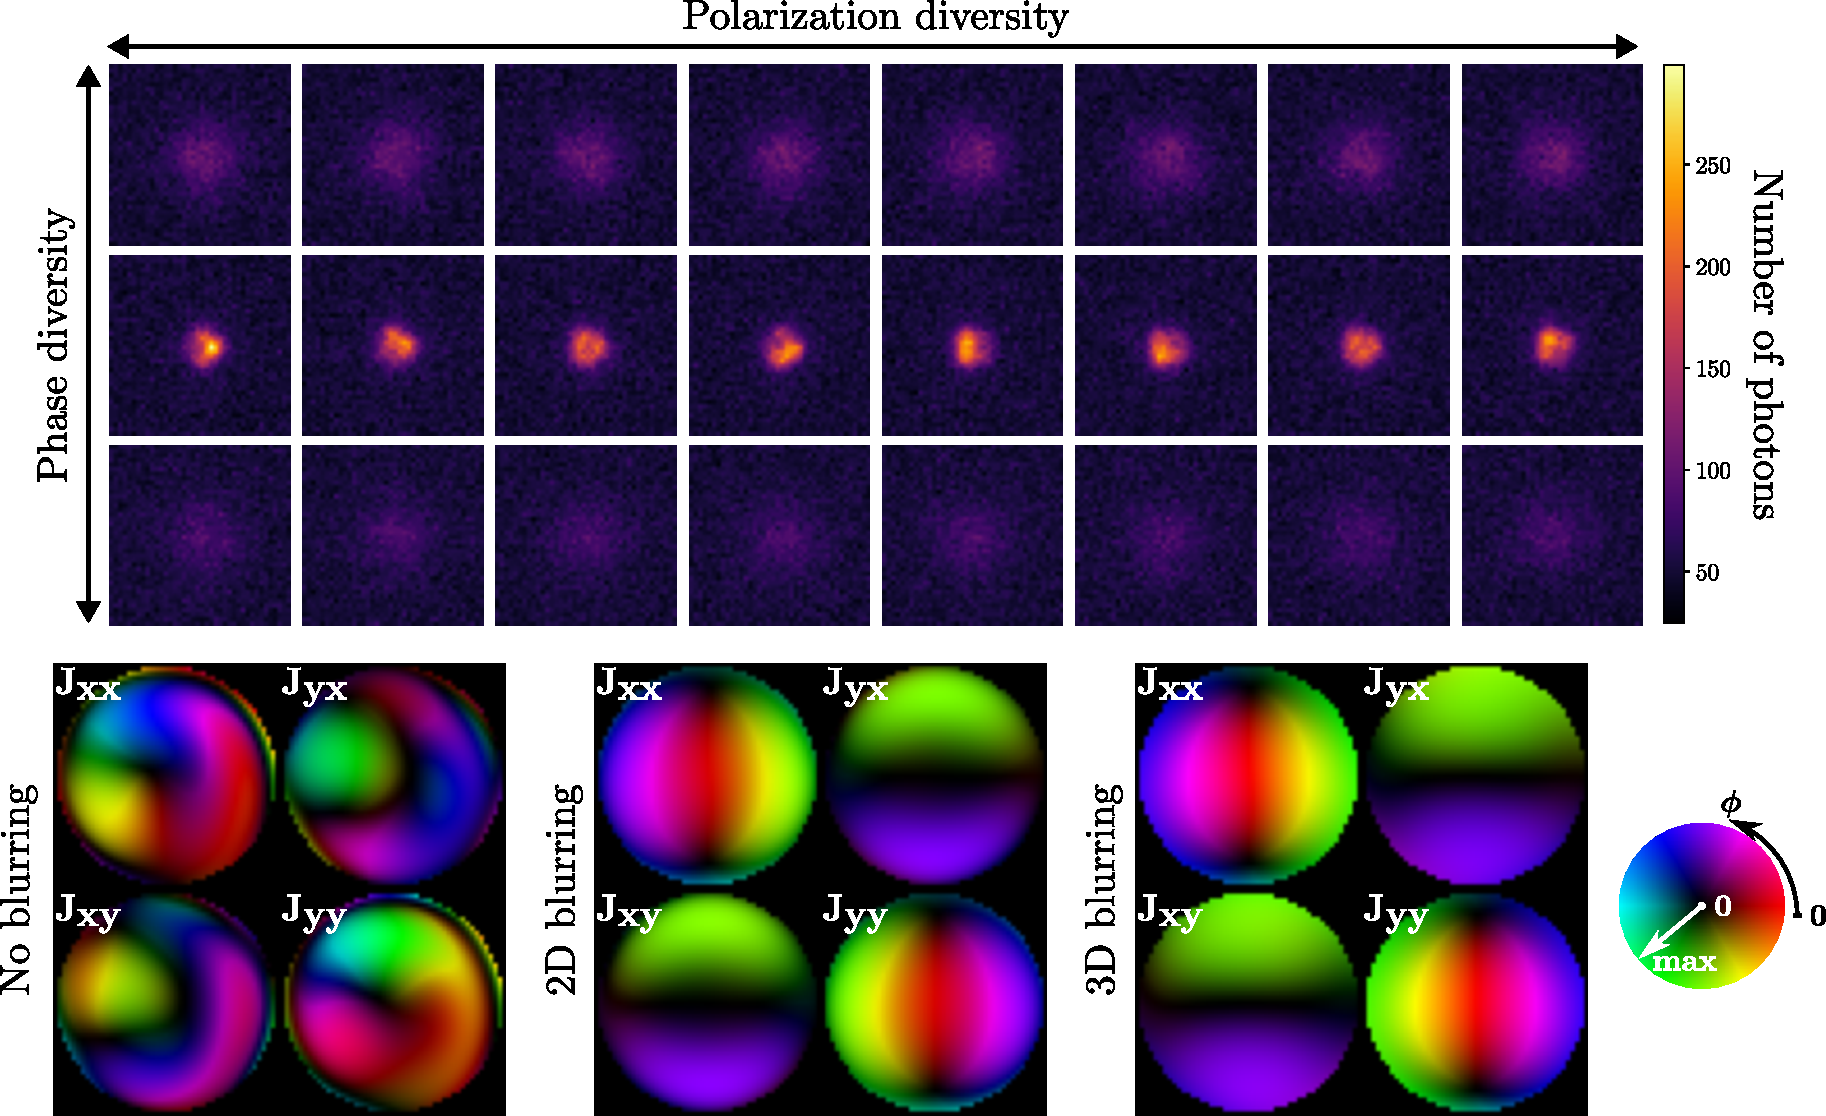
\includegraphics[width=1.\linewidth]{blurring.pdf}
  \caption{\label{fig:qp_ret} . }
\end{figure}

In order to showcase the implementation of blurring in our model, we now consider a 
200nm fluorescent nanobead which produces blurred PSFs due to its size. Let us only treat 
the SEO birefringent mask with the same choice of phase and polarization 
diversities as before.


\section{Characterizing the polarization aberrations in an experimental
setup}




%\section{Numerical simulations}
%
%\subsection{Test cases}
%
%\begin{itemize}
%\item Standard scalar aberrations
%\item Standard polarization and scalar aberrations
%\item S-plate
%\item Birefringent window (SEO)
%\end{itemize}
%
%\subsection{Scalar VS polarization aberrations}
%
%Our model allows us to turn off and on the coefficients used for the 
% Zernike decomposition. In particular, the decomposition for the Jones 
% matrix in terms of Pauli matrices allows us to consider purely scalar 
% aberrations. Here, we explore how well purely scalar aberrations perform 
% particularly when fitting high amounts of birefringent such as those used 
% for PSF engineering. 
%
%
%\subsection{•}
%
%
%\section{Cross validation and the importance of polarization diversity}
%
%Due to experimental constraints we assumed that the source used for the characterization of the system emitted unpolarized light. This is in line with most common scenarios that use fluorescent nano-beads. However, when using the setup for a real measurement, the individual fluorophores emit light that depends on the amount of wobble. If the fluorophare stays fixed within  the acquisition time window, then it will emit light as a fully coherent dipole. 
%Given that the phase retrieval was done with unpolarized light, in order to test the accuracy of the model we run it on a cross-validation set of dipole with different orientations, at different focal planes and distance from the cover-slip. 
%





\begin{acknowledgments}
S. Paine for useful discussions.
\end{acknowledgments}

%% The Appendices part is started with the command
 \appendix

\section{Expressions for the Green tensor at the BFP}

As outlined in \cite{novotny2006principles}, a closed-form for the Green tensor at the BFP for a dipolar source placed close to an interface can be obtained. In particular the components of the $\bt g$  tensor in Eq.~(\ref{eq:green}) are given by
\begin{widetext}
\begin{align}
\bt g(\bt u) =\frac{1}{(1-u^2)^{1/4}} \left( 
\begin{array}{ccc}
\cos^2 \phi \sqrt{1-u^2} \Phi_2 + \sin^2 \phi \Phi_3 & \cos \phi \sin \phi ( \sqrt{1-u^2} \Phi_2 - \Phi_3) & -u \cos \phi \Phi_1  \\
\cos \phi \sin \phi ( \sqrt{1-u^2} \Phi_2 - \Phi_3) &  \sin^2 \phi \sqrt{1-u^2} \Phi_2 + \cos^2 \phi \Phi_3 & - u \sin  \phi \Phi_1
\end{array}
\right).
\end{align}
\end{widetext}
%\bse
%\begin{align}
%g_{11} =& \cos^2 \phi \sqrt{1-u^2} \Phi_2 + \sin^2 \phi \Phi_3  \\
%g_{12}=& \cos \phi \sin \phi ( \sqrt{1-u^2} \Phi_2 - \Phi_3) \\
%g_{13}=& -u \cos \phi \Phi_1 \\
%g_{21}=& g_{12} \\
%g_{22}=& \sin^2 \phi \sqrt{1-u^2} \Phi_2 + \cos^2 \phi \Phi_3 \\
%g_{23}=& - u \sin  \phi \Phi_1.
%\end{align}
%\ese
where 
\bse
\begin{align}
\Phi_1(u) = & t^p(u) \frac{n_i k_i\sqrt{1-u^2} }{n_m \sqrt{k_m^2 -k_i^2 u^2}} \\
\Phi_2(u) = & t^p(u)\frac{n_i}{n_m} \\
\Phi_3(u) = & t^s(u) \frac{k_i \sqrt{1-u^2}}{\sqrt{k_m^2 -k_i^2 u^2}}
\end{align}
\ese
with
\bse
\begin{align}
t^s(u) = & \frac{2k_{m,z}}{k_{m,z} + k_{i,z}},\\
t^p(u) = &  \frac{n_m}{n_i}\frac{2n_i^2 k_{m,z}}{n_i^2 k_{m,z} + n_m^2 k_{i,z}}.
\end{align}
\ese
being the Fresnel coefficients for p and s polarized light.


%\bibliography{Refs-raysNwaves}
\bibliography{microscopy}



\end{document}



